% ============================================================
% 片段：s04b  对应原文 section2.tex 第 1198--1468 行；PDF 第 43--49 页
% 内容：§4.2 在凝聚态物理中的应用（4.2.1 环面码模型；4.2.2 3+1 维的 SPT）
% 译者：t-s04b   审校状态：初稿
% ============================================================

% ==== 原文 PDF 第 43 页 ====
\subsection{在凝聚态物理中的应用}\label{sec:appl-CMP}

研究广义对称性的一个自然框架，由具有任意子激发的 2+1 维拓扑序提供；这些系统在凝聚态物理领域已被广泛研究。它们在数学上由幺正模张量范畴描述，后者为刻画任意子的融合与编织结构提供了强有力的形式体系\cite{KITAEV20062}。这些系统中任意子所扫出的世界线，可以解释为该系统的拓扑缺陷线（topological defect line，TDL）。这类算符的关键之处在于：与作用于整个系统的整体对称性作用不同，它们只作用于系统中一部分自由度\cite{PhysRevB.72.045137,pnas.0803726105,NUSSINOV2009977}。在这个意义上，它是逐点作用于系统的规范对称变换的推广。

当任意子为阿贝尔任意子时，系统中的所有 TDL 都是可逆的。此时，由任意子世界线生成的对称性对应于 1-形式对称性。反之，若任意子是非阿贝尔的（这意味着 TDL 非可逆），则与任意子世界线相联系的对称性就是非可逆对称性。

为说明这些概念，我们以著名的环面码模型（toric code model）作为具体例子。我们将证明，这个 2+1 维系统中由任意子世界线产生的 1-形式对称性是反常的。此外，我们还将说明，这个带有反常 1-形式对称性的系统可以作为 3+1 维 1-形式 SPT 态的边界而被实现。

\subsubsection{环面码模型}

环面码模型\cite{KITAEV20032}是规范群为 $\mathbb{Z}_2$ 的 2+1 维格点规范理论的一个著名例子。该模型中，我们考虑具有正方格子的二维空间，其中每条格点边（link）都赋予一个自旋-$1/2$ 自由度。系统的希尔伯特空间是每条边对应的复二维向量空间 $\mathbb{C}^2$ 的张量积：
\be
\mathcal{H} = \bigotimes_{\text{每条边}} \mathbb{C}^2.
\ee

我们在环面码模型中定义如下两类算符：
\begin{center}
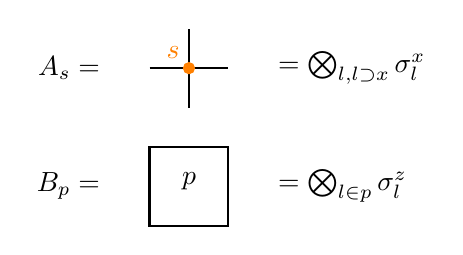
\begin{tikzpicture}
    \draw[thick] (-0.5,0)--(0.5,0) (-1,0)node[left]{$A_s = $};
    \draw[thick] (0,-0.5)--(0,0.5) (1,0) node[right]{$ = \bigotimes_{l, \ptl l\supset {x}} \sigma^{x}_{l}$};
    \filldraw[orange] (0,0) circle (2pt) (-0.2,0)node[above]{$s$};
    \draw[thick] (-0.5,-2) rectangle (0.5,-1) (-1,-1.5)node[left]{$B_p = $} (0,-1.2)node[below]{$p$} (1,-1.5)node[right]{$ = \bigotimes_{ l\in \ptl p} \sigma^{z}_{l}$};
\end{tikzpicture}
\end{center}

其中每个顶点（vertex）记为 $s$，每个面（plaquette）记为 $p$。
% ==== 原文 PDF 第 44 页 ====
不难验证这些算符具有如下性质
\be\ba 
A_s^\dag &= A_s,  \ \ A_s^2 = 1 \Rightarrow \ {\rm Spec}(A_s) = {\pm 1} ,\\ 
B_p^\dag &= B_p, \ \ B_p^2 = 1 \Rightarrow \ {\rm Spec}(B_p) = {\pm 1} ,\\
[A_s,A_{s'}] &= [B_p,B_{p'}]= [A_s,B_p]  = 0 , \ \forall s,s',p,p' .
\ea\ee

环面码模型的哈密顿量是与 $A_s$ 及 $B_p$ 算符相关联的所有相互对易的投影算符项之和，即：
\be
H = -\left(\sum_{s} A_s + \sum_{p} B_p\right).
\ee

由于哈密顿量中所有项彼此对易，我们可以容易地确定该模型的全部能谱：
\be\ba
\text{基态} &:  A_s\ket{0} = B_p\ket{0} = \ket{0} \\
\text{激发态} &: A_s \ket{\Psi} = -\ket{\Psi}, \text{ 或 } B_p \ket{\Psi} = -\ket{\Psi},  \ \text{对某些 }s,p
\ea\ee

这简化了寻找基态与激发态的过程，使得分析环面码模型的行为并研究其激发变得可行。

环面码模型与电磁学之间存在直观的对应关系，后者由 $U(1)$（格点）规范理论描述。
\begin{center}
    \begin{tabular}{ccc}
        离散 $\bbZ_2$ 规范理论 & $\longrightarrow$  &  $U(1)$ 规范理论  \\
        $\sigma^z_l$ &   $\longrightarrow$  &  威尔逊线 $\exp(i\int A_{ij})$  \\
        $B_p$ &   $\longrightarrow$  &  $\exp(i\oint A)=  \exp(i\int F) \sim \exp(ia^2 B) $  \\
        $\sigma^x_{l}$ &   $\longrightarrow$  &  $\exp(i\int_l E)$  \\
        $A_s$ &   $\longrightarrow$  & $\exp(i \nabla\cdot E)$   \\
        $H = -(\sum_s A + \sum_p B)$ &   $\longrightarrow$  &  $\vb{B}^2 + (\nabla\cdot \vb{E})^2$  \\
        $B_p = \pm 1$ &  $\longrightarrow$   &  $ \int B =0 \ / \ \ne 0$  \\
        $A_s = \pm 1$ &   $\longrightarrow$  &  $\nabla E = 0\ / \ \ne 0$  \\

    \end{tabular}
    \label{tab:Z2U1}
\end{center}

\begin{yizhu}该表是“离散 $\Z_2$ 规范理论与连续 $U(1)$ 规范理论”之间的对照词典，读表时须分清两类角色：开弦 $\sigma^z_l$ 对应威尔逊线，按 (4.21) 它是 $\Z_{2,M}^{(1)}$ 的带荷对象；与它对偶的 't Hooft 线 $\sigma^x_{l}$ 则是 $\Z_{2,E}^{(1)}$ 的带荷对象。而闭圈 $B_p$ 与 $A_s$ 分别是 $\Z_{2,E}^{(1)}$、$\Z_{2,M}^{(1)}$ 的对称性算符：由 (4.14) 可见 $B_p$ 只与 $W_M$ 的端点（$p\in\partial L^\ast$ 处）反对易，$A_s$ 只与 $W_E$ 的端点（$s\in\partial L$ 处）反对易。表中 $B_p$ 一行写作 $\exp(i\oint A)$（闭威尔逊圈，而不是威尔逊线）并等价于 $\exp(ia^2B)$，正是这一对偶互换的体现：在环面码中，一个 1-形式对称性的生成元恰是另一个 1-形式对称性的带荷算符。\end{yizhu}

这一对应关系还有助于我们构造环面码模型中的激发。1-形式对称性可以通过与这些激发相联系的弦算符（string operator）来理解，如下图所示：

% ==== 原文 PDF 第 45 页 ====
\begin{center}
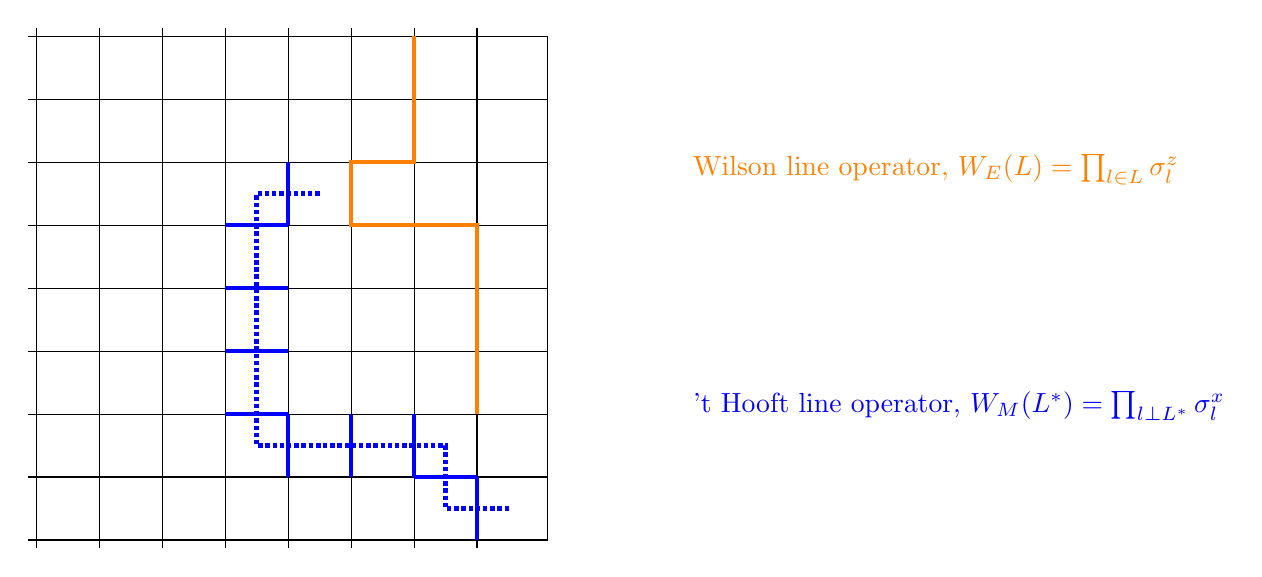
\begin{tikzpicture}
    \draw[] (-3.3,3.2)--(3.3,3.2);
    \draw[shift = {(0,-0.8)}] (-3.3,3.2)--(3.3,3.2);
    \draw[shift = {(0,-1.6)}] (-3.3,3.2)--(3.3,3.2);
    \draw[shift = {(0,-2.4)}] (-3.3,3.2)--(3.3,3.2);
    \draw[shift = {(0,-3.2)}] (-3.3,3.2)--(3.3,3.2);
    \draw[shift = {(0,-4.0)}](-3.3,3.2)--(3.3,3.2);
    \draw[shift = {(0,-4.8)}](-3.3,3.2)--(3.3,3.2);
    \draw[shift = {(0,-5.6)}](-3.3,3.2)--(3.3,3.2);
    \draw[shift = {(0,-6.4)}](-3.3,3.2)--(3.3,3.2);
    \draw[] (3.3,-3.2)--(3.3,3.2);
    \draw[shift = {(-0.8,0)}] (3.2,-3.3)--(3.2,3.3);
    \draw[shift = {(-1.6,0)}] (3.2,-3.3)--(3.2,3.3);
    \draw[shift = {(-2.4,0)}] (3.2,-3.3)--(3.2,3.3);
    \draw[shift = {(-3.2,0)}] (3.2,-3.3)--(3.2,3.3);
    \draw[shift = {(-4.0,0)}] (3.2,-3.3)--(3.2,3.3);
    \draw[shift = {(-4.8,0)}] (3.2,-3.3)--(3.2,3.3);
    \draw[shift = {(-5.6,0)}] (3.2,-3.3)--(3.2,3.3);
    \draw[shift = {(-6.4,0)}] (3.2,-3.3)--(3.2,3.3);
    \draw[orange, ultra thick]  (1.6,3.2)--(1.6,2.4)--(1.6,1.6)--(0.8,1.6)--(0.8,0.8)--(1.6,0.8)--(2.4,0.8)--(2.4,-1.6) (5,1.5)node[right]{Wilson line operator, $W_E(L) = \prod_{l\in L} \sigma^z_l  $};
    \draw[blue,ultra thick, densely dotted] (0.4,1.2)--(-0.4,1.2)--(-0.4,0.4)--(-0.4,-0.4)--(-0.4,-1.2)--(-0.4,-2.0)--(0.4,-2.0)--(1.2,-2.0)--(2.0,-2.0)--(2.0,-2.8)--(2.8,-2.8);
    \draw[blue,ultra thick] (0,0.8)--(0,1.6)     (5,-1.5)node[right]{'t Hooft line operator, $W_M(L^*) = \prod_{l\perp L^*} \sigma^x_l$};
    \draw[blue,ultra thick] (0,0.8)--(-0.8,0.8);
    \draw[shift = {(0,-0.8)},blue,ultra thick] (0,0.8)--(-0.8,0.8);
    \draw[shift = {(0,-1.6)},blue,ultra thick] (0,0.8)--(-0.8,0.8);
    \draw[shift = {(0,-2.4)},blue,ultra thick] (0,0.8)--(-0.8,0.8);
    \draw[shift = {(2.4,-3.2)},blue,ultra thick] (0,0.8)--(-0.8,0.8);

    \draw[shift = {(0,-3.2)},blue,ultra thick] (0,0.8)--(0,1.6);
    \draw[shift = {(0.8,-3.2)},blue,ultra thick] (0,0.8)--(0,1.6);
    \draw[shift = {(1.6,-3.2)},blue,ultra thick] (0,0.8)--(0,1.6);
    \draw[shift = {(2.4,-4)},blue,ultra thick] (0,0.8)--(0,1.6) ;
    
\end{tikzpicture}
\end{center}

在如上定义了威尔逊线与 't Hooft 线算符之后，可以证明它们的对易子为（当存在非零交点时）
\be\ba
[ W_E(L), B_p ] &= 0,  \ \ [W_M(L^*),B_p]\ne 0 \text{ iff } p\in\partial L^\ast \\
[W_E(L),A_s]&\ne 0 \text{ iff }s\in \partial L, \ \ [W_M(L^*), A_s] = 0  \\
[W_E(L) ,H] &= [W_M(L^*),H] = 0 \ {\rm if} \ \ptl L = \partial L^\ast=  0\\
[W_E(L), W_M(L^*) ] &= 0  \ , \ {\rm if \ } L \cap L^\ast = 0 
\ea\ee

现在可以陈述如下事实：\textbf{环面码系统的激发是开线算符的端点。}更具体地，有
\be
 \ba
s &\notin \ptl L \  : \ A_s W_E(L) \ket{0} = W_E(L) A_s \ket{0} =  W_E(L) \ket{0} \\
s &\in \ptl L \ : \ A_s W_E(L) \ket{0} = -W_E(L) A_s \ket{0} =  -W_E(L) \ket{0}
\ea  \ee

因此，电荷 $e$ 是威尔逊线的端点。类似地，对磁的部分，有
\be
 \ba
p &\notin \ptl L^* \  : \ B_p W_M(L) \ket{0} = W_M(L^*) B_p \ket{0} =  W_M(L^*) \ket{0} \\
p &\in \ptl L^* \ : \ B_p W_M(L) \ket{0} = -W_M(L^*) B_p \ket{0} =  -W_M(L^*) \ket{0}
\ea   \ee

因此，磁荷 $m$ 是 't Hooft 线端点处的激发。

与开线给出激发的情形相反，闭圈是用于对简并态分类的守恒荷。我们关心的是基态。设该格点的整体结构为环面 $T^2 = S^1\times S^1$，则有两类非平凡圈。考虑 $W_E(L_{1,2}) = \pm 1$ 或 $W_M(L_{1,2})=\pm 1$，简并度至少为 4。

\begin{yizhu}基态简并度“至少为 4”的理由可用逻辑算符来说明：在 $T^2$ 上，$W_E$ 与 $W_M$ 各有两个不可收缩的闭圈，即 $W_E(L_1),W_E(L_2)$ 与 $W_M(L_1^\ast),W_M(L_2^\ast)$；它们都与 $H$ 对易，但电型闭圈与磁型闭圈之间互不对易，且 $W_E^2=W_M^2=1$。因此在基态子空间上可以同时取两组独立的 $\pm1$ 本征值，给出 $2^2=4$ 维基态空间；对亏格 $g$ 的曲面应推广为 $2^{2g}$。注意这些闭圈正是非定域的逻辑算符，与开弦端点处的任意子激发 $e$、$m$、$em$ 是不同对象。\end{yizhu}

通过在二维空间流形的希尔伯特空间上对泡利矩阵作简单计算，可以看出
\be\label{EM} W_E(L) W_M(L^*) = (-1)^{{\rm Int}(L,L^*)}   W_M(L^*)W_E(L), \ee

这意味着 't Hooft 线是威尔逊线所作用的对象，反之亦然。这里 $\mathrm{Int}(L,L^\ast)$ 是二维空间流形上两条线 $L$ 与 $L^\ast$ 的交点数。至此，我们已准备好讨论激发的统计性质。

% ==== 原文 PDF 第 46 页 ====
若同时考虑时间维度，这些线现在便画在 2+1 维时空之中。由于沿同一链的 $\sigma_l^x$ 与 $\sigma_l^z$ 反对易，交换两条线的次序会产生一个负号。这一概念可用下图直观地表示：
\begin{center}
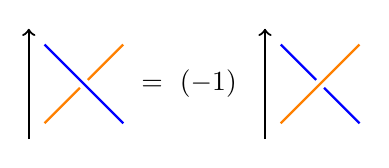
\begin{tikzpicture}
    \draw[orange , thick ] (0,0)--(0.45,0.45)  (0.55,0.55)--(1,1);
    \draw[blue, thick]  (1,0)--(0,1);
    \draw[thick , -> ] (-0.2,-0.2)--(-0.2,1.2);
    \draw[thick] (-0.2,0)--(-0.2,1) (1.1,0.5)node[ right]{$= \ (-1)$};
    \draw[shift = {(3,0)},thick , -> ] (-0.2,-0.2)--(-0.2,1.2);
    \draw[shift = {(3,0)},orange ,thick] (0,0)--(1,1);
    \draw[shift = {(3,0)},blue, thick] (0,1)--(0.45,0.55) (0.55,0.45)--(1,0);
\end{tikzpicture}
\end{center}

这蕴含着该系统的阿哈罗诺夫–玻姆效应（Aharonov-Bohm effect）
\begin{center}
    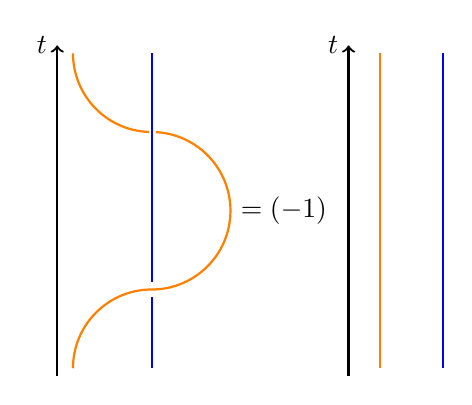
\begin{tikzpicture}
        \draw[thick,->] (-0.20,-0.1)--(-0.20,4.1) node[left]{$t$};
        \draw[shift = {(3.7,0)},thick,->] (-0.20,-0.1)--(-0.20,4.1) node[left]{$t$};

        \draw[thick] (-0.20,0)--(-0.20,1) (2,2)node[right]{$= (-1)$};
        \draw[orange,thick] (0,0) arc (180:90:1) (1,1) arc (-90:87:1) (0,4) arc (180:268:1);
        \draw[thick, blue] (1,0)--(1,0.9) (1,1.1)--(1,4);
        \draw[shift = {(3.7,0)},thick, blue] (1,0)--(1,4) ;
        \draw[shift = {(3.7,0)},thick, orange] (0.2,0)--(0.2,4) ;

    \end{tikzpicture}.
\end{center}

以及，如果把线的端点闭合成圈，一个 Hopf 链环的取值：
\begin{center}
    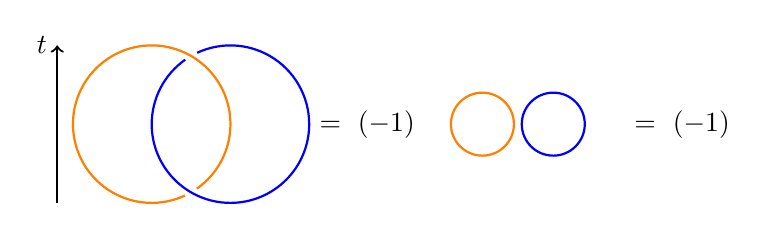
\begin{tikzpicture}
        \draw[thick , orange] (1,0) arc (0:295:1) (1,0) arc (0:-55:1) ;
        \draw[thick , blue] (2,0) arc (0:-235:1) (2,0) arc (0:115:1);
        \draw[thick,->] (-1.2,-1)--(-1.2,1) node[left]{$t$};
        \draw[thick] (-1.2,0)--(-1.2,0.1) (2.0,0) node[right]{$= \ (-1)$} (6,0) node[right]{$= \ (-1)$} ;
        \draw[shift = {(1.6,0)},thick , orange] (3,0) arc (0:360:0.4) ;
        \draw[shift = {(2,0)},thick , blue] (3.5,0) arc (0:360:0.4) ;
      
    \end{tikzpicture}
\end{center}


从高形式对称性的角度看，2+1 维环面码模型显然具有 $\mathbb{Z}_{2,E} \times \mathbb{Z}_{2,M}$ 1-形式对称性，其特征如下：
\be\ba
\bbZ_{2,E}^{(1)}: W_E(L) W_M(L^*) &= (-1)^{{\rm Link}(L,L^*)}  W_M(L^*), \\
\bbZ_{2,M}^{(1)}: W_M(L^\ast) W_E(L) &= (-1)^{{\rm Link}(L^\ast,L)}  W_E(L) .
\ea\ee

这些方程应在 2+1 维时空的语境下理解，而不是如式~(\ref{EM}) 那样在二维空间的语境下理解。值得注意的是，对这两个不同的 1-形式对称性而言，威尔逊线算符与 't Hooft 线算符的角色可以互换：一个充当 1-形式对称性算符，另一个则是其带荷算符。

\begin{yizhu}(4.14) 与 (4.17) 的对易关系是弦算符与格点算符作用次序的直接推论：$W_E(L)$ 是沿链 $L$ 的 $\sigma^z_l$ 之积，因此只有当 $A_s=\prod_{l\ni s}\sigma^x_l$ 的支撑与 $L$ 在端点 $s\in\partial L$ 处重叠时才会出现反对易；同理，$W_M(L^\ast)$ 只在 $p\in\partial L^\ast$ 处与 $B_p$ 反对易。所有 $(-1)$ 因子的唯一来源是同一链上 $\sigma_l^x\sigma_l^z=-\sigma_l^z\sigma_l^x$，即每条边上的自旋-$1/2$ 自由度，这也解释了为何这些对易子只能取 $\pm1$。另须注意维数：(4.17) 写在二维空间中，因子是 $(-1)^{\mathrm{Int}(L,L^\ast)}$；而 (4.18) 写在 2+1 维时空中，因子是 $(-1)^{\mathrm{Link}(L,L^\ast)}$。把其中一条线提升为时间方向的世界线后，二者是同一个拓扑量，但对易子的计算语境不可混用。\end{yizhu}

% ==== 原文 PDF 第 47 页 ====
这把我们引向该 1-形式对称性的反常问题。事实上，这两个 $\Z_2$ 1-形式对称性具有混合 't Hooft 反常。它可以从三个不同视角来理解：
\begin{enumerate}
    \item 威尔逊圈与 't Hooft 圈在 2+1 维时空中的构型，对应于 1-形式对称性的一个缺陷网络。由于这两个 $\Z_2$ 1-形式对称性彼此不同，它们的缺陷线应当保持相互独立。然而，如前文所讨论的，该缺陷网络在本质上不是拓扑的：
    \be
    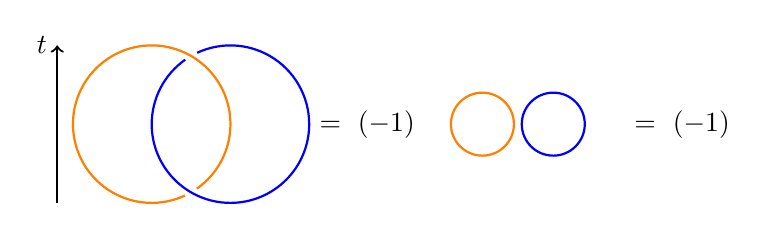
\begin{tikzpicture}
    \label{grf:link}
        \draw[thick , orange] (1,0) arc (0:295:1) (1,0) arc (0:-55:1) ;
        \draw[thick , blue] (2,0) arc (0:-235:1) (2,0) arc (0:115:1);
        \draw[thick,->] (-1.2,-1)--(-1.2,1) node[left]{$t$};
        \draw[thick] (-1.2,0)--(-1.2,0.1) (2.0,0) node[right]{$= \ (-1)$} (6,0) node[right]{$= \ (-1)$} ;
        \draw[shift = {(1.6,0)},thick , orange] (3,0) arc (0:360:0.4) ;
        \draw[shift = {(2,0)},thick , blue] (3.5,0) arc (0:360:0.4) ;
      
    \end{tikzpicture}
\ee
    这一现象可以理解为一种混合反常，类似于前文提到的 1+1 维情形中结合律的破坏。
    \item 另一个考察反常的视角是通过规范变换。环面码的作用量可以写成一个陈–西蒙斯理论
    \be S = \int_{M_3}  \frac{2}{2\pi} b^{(1)}\wedge \dd a^{(1)}  \ee
    其中威尔逊线与 't Hooft 线算符为
    \be\left\{ \ba
    W_E(L) &= \exp(i\int_L a),  \ \ \ \ \bbZ_{2,M}^{(1)}\ \text{带荷算符} \\
    W_M(L) &= \exp(i\int_L b), \ \  \ \ \bbZ_{2,E}^{(1)}\ \text{带荷算符} 
    \ea \right. \ee
    现在，若把该理论与背景 2-形式规范场（记为 $B_{E,M}^{(2)}$）耦合，试图对 $\bbZ_{2,E}^{(1)}\times \bbZ_{2,M}^{(1)}$ 1-形式对称性作规范化，则得到如下作用量
    \be S = \int_{M_3}  \frac{2}{2\pi} b^{(1)}\wedge \dd a^{(1)}  + \int_{M_3} \frac{1}{2\pi} (a^{(1)}\wedge B_M^{(2)}+ b^{(1)}\wedge B_E^{(2)}). \ee
    在 $\bbZ_{2,E}^{(1)}$ 规范变换
    \be\left \{ \ba
    B_E &\mapsto B_E - \dd \chi \\
    a &\mapsto a+ \frac{1}{2} \chi 
    \ea \right. \ee
    之下，由于第二项，作用量显然不是规范不变的，尽管其余两项保持不变。类似地，对磁规范变换，
% ==== 原文 PDF 第 48 页 ====
    作用量也同样缺乏规范不变性。然而，若把该理论与一个 3+1 维体（bulk）耦合，其作用量为
    \be\label{eq:Sbulk} S_{\rm bulk} = \frac{1}{4\pi^2}\int_{M_4} B_E \wedge B_M, \ee
    则发现总理论变为规范不变的，这表明两个 1-形式对称性的混合反常由高一维的上述反常多项式所支配。
    \item 从分类空间的视角看，把两个规范场视为从时空到分类空间的映射：
    \be B,B': M_3 \to B^2(\bbZ_{2,E}\times \bbZ_{2,M} ) \ .\ee
    设这两个规范场映射分别对应于式~\ref{grf:link} 中非平凡链环与平凡链环的左右两侧缺陷网络构型。由于这两个 1-形式对称性彼此独立，两种构型的映射是同伦的。在无反常的理论中，两种构型的配分函数应当相同。然而在此情形下，式~\ref{grf:link} 中两种构型的配分函数相差一个 $(-1)$ 因子，这标志着混合反常的存在。
\end{enumerate}

\subsubsection{3+1 维的 $\bbZ_{2,E}^{(1)}\times \bbZ_{2,M}^{(1)}$ SPT}

为深化对前述 $\bbZ_{2,E}\times \bbZ_{2,M}$ 1-形式对称性反常的理解，可以尝试从 3+1 维 1-形式 SPT 的视角来认识它。3+1 维 $\bbZ_{2,E}^{(1)}\times \bbZ_{2,M}^{(1)}$ SPT 由下式分类
\be\ba  
H^4( B^2 \bbZ_{2,E}\times  B^2\bbZ_{2,M} ,U(1)) &\supset H^2(B^2 \bbZ_{2,E} , H^2( B^2\bbZ_{2,M} , U(1))) \\
&\cong  H^2(B^2 \bbZ_{2,E} ,\bbZ_2) \cong \bbZ_2 .
\ea\ee

它是上同调群的谱序列计算中的一项。值得注意的是，这一 $\bbZ_2$ 分类由项 $B_E^{(2)}\wedge B_M^{(2)}$ 生成。由此得到的 3+1 维 SPT 作用量表示为：
\be S_\mathrm{SPT} = \frac{1}{4\pi^2}\int_{M_4} B_E \wedge B_M.  \ee

这一结果恰好印证了式~(\ref{eq:Sbulk}) 中详述的反常多项式方法。本质上，它再次确认：2+1 维中两个 1-形式对称性的混合反常，可以通过由两个 2-形式规范场之楔积所刻画的 3+1 维 SPT 来理解。

\begin{yizhu}(4.26) 是上同调群的谱序列计算中的一项：对 $G=B^2\bbZ_{2,E}\times B^2\bbZ_{2,M}$，$H^4(BG,U(1))$ 由 Leray（Atiyah–Hirzebruch）谱序列的 $E_2^{p,q}=H^p(B^2\bbZ_{2,E},H^q(B^2\bbZ_{2,M},U(1)))$ 项逼近，作者给出的是 $p=q=2$ 这一项，即 $H^2(B^2\bbZ_{2,E},\bbZ_2)\cong\bbZ_2$，它由 $B_E^{(2)}\wedge B_M^{(2)}$ 生成。这里的 $\supset$ 表示它只是整个 $H^4$ 的一部分，其余 $(p,q)$ 项一般还可给出别的分类项；本例中该 SPT 的完整分类恰为 $\bbZ_2$。此外，$S=\frac{1}{4\pi^2}\int_{M_4}B_E\wedge B_M$ 的归一化要求 $B_{E,M}$ 是 $U(1)$ 联络的场强，即 $\oint B\in2\pi\bbZ$；在此归一化下 $\exp(iS_{\rm SPT})=(-1)^{nm}$，其中 $n,m$ 分别是 $B_E$、$B_M$ 在两个对偶 2-闭链上的通量整数。核对时应与 (4.22) 中的 $\frac{1}{2\pi}$ 耦合系数一并检查。\end{yizhu}

% ==== 原文 PDF 第 49 页 ====
现在，我们从拓扑缺陷网络的观点来考察：体作用量与边界作用量的反常为何相互抵消。2+1 维中的线算符可以自然地延拓为 3+1 维体中的面算符。由于总时空维数为四，两个这样的面算符的交集出现在 3+1 维时空中的离散点处。应用庞加莱对偶（Poincaré duality），这一交集可以等价地理解为 $B_E$ 与 $B_M$ 楔积的积分：
\be  B_E\wedge B_M \stack{\text{Poincar\'{e} 对偶}}{\longleftrightarrow} S_E\cap S_M. \ee

因此，3+1 维 1-形式 SPT 的作用量本质上是在数两个与 2-形式规范场对偶的面之间交点数的奇偶性。

这一几何解释漂亮地阐明了体与边界作用量之间反常的抵消。事实上，当我们试图把 2+1 维时空中的一个 Hopf 链环构型（如式~\ref{grf:link} 左侧所示）延拓到高一维时，最直接的延拓是到 4+1 维中的一个面，这将涉及单个交点。按此几何推理，体与边界理论合并后的整体是无反常的：
\be  (-1)^{\text{3+1 维中的交点数}} \cdot (-1)^{\text{2+1 维中的环绕数}} = 1.  \  \ee

由这一视角，我们完全从几何上理解了反常的抵消。

\begin{center}
    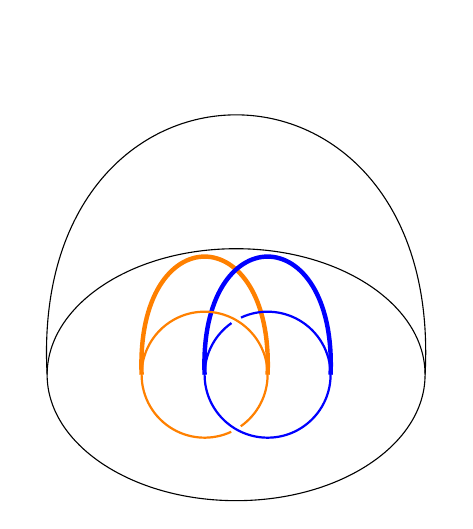
\begin{tikzpicture}[scale = 0.8]
        \draw (0.5,0) ellipse (3 and 2);
        \draw[shift = {(0.5,0)}] (-3,0) .. controls (-3.3, 5.5) and (3.3,5.5) .. (3,0);
        \draw[ultra thick, orange] (-1,0) .. controls (-1.1,2.5) and (1.1,2.5) .. (1,0);
        \draw[shift = {(1,0)},ultra thick, blue] (-1,0) .. controls (-1.1,2.5) and (1.1,2.5) .. (1,0);

        \draw[thick , orange] (1,0) arc (0:295:1) (1,0) arc (0:-55:1) ;
        \draw[thick , blue] (2,0) arc (0:-235:1) (2,0) arc (0:115:1);

    \end{tikzpicture}
\end{center}

还可以通过考察 1-形式 SPT 及其边界模型的具体格点模型来进一步加深理解。这使我们能够更细致地研究体对称性算符如何与边界算符相互作用，以及反常抵消如何发生。关于 $\mathbb{Z}_N$ 1-形式对称性的一个示例见文献\cite{PhysRevB.101.035101}。

\begin{yizhu}[原文疑误]原文此处写“the most straightforward extension to a surface in 4+1D”，与同段 (4.29) 中的“3+1D”以及全节始终在 3+1 维体中讨论的事实不一致：2+1 维时空中的两条线延拓一维后是 3+1 维时空中的两个面，而正是两个面在 3+1 维时空中才一般交于离散点（若真到 4+1 维，两个面一般交于 1 维曲线，不会给出“单个交点”）。此处照原文保留“4+1D”，疑应为“3+1D”。\end{yizhu}

% ==== 原文 PDF 第 49 页内容至此结束；第 50 页起为第 5 节（属其他片段）====
